\chapter{Thiết kế Sentinel Pulse}

Pulse có hai nhánh phát hiện chạy song song trên cùng số đếm syscall: một model ML theo workload và một luật tripwire. Bất kỳ nhánh nào báo cũng sinh cảnh báo; RCA dựng cây bằng chứng cho mỗi cảnh báo đã gửi đi.

\begin{figure}[htbp]
  \centering
  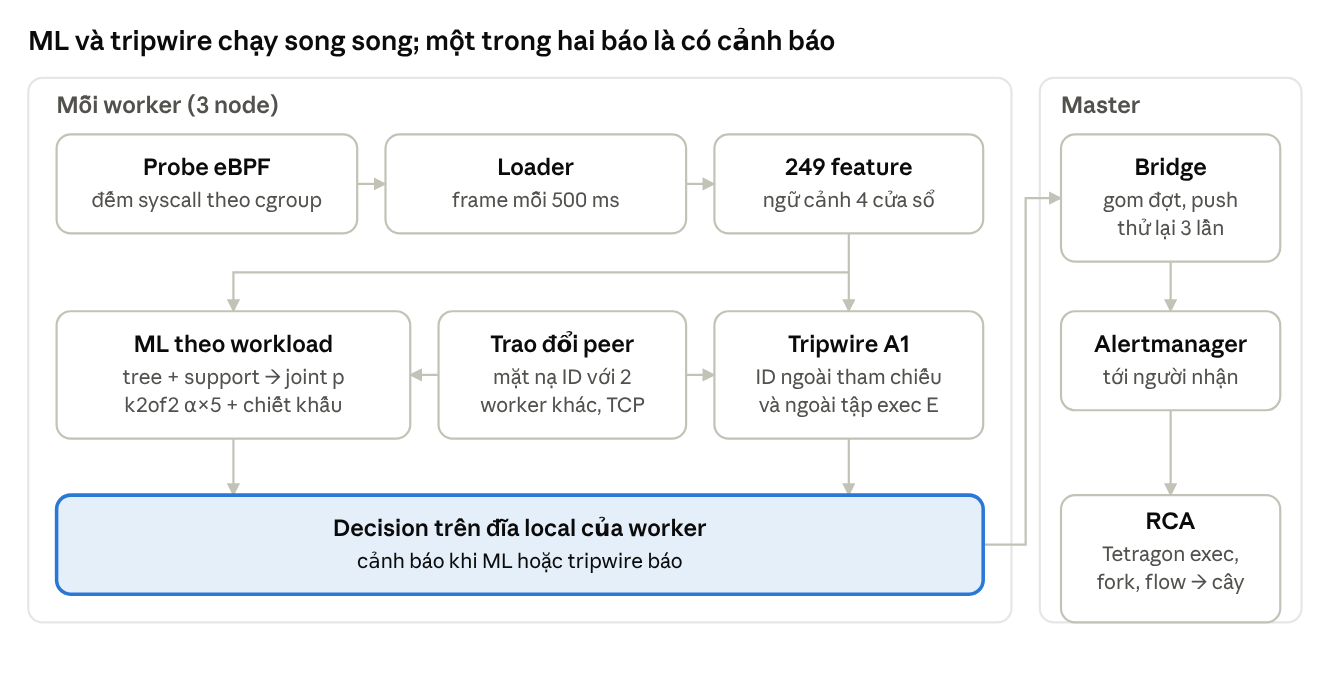
\includegraphics[width=\linewidth]{architecture.png}
  \caption{Kiến trúc Sentinel Pulse (hệ thống cuối, lượt \texttt{pulse-\allowbreak{}final-\allowbreak{}system-\allowbreak{}confirm}).}
  \label{fig:architecture}
\end{figure}

Trên mỗi worker, ML và tripwire cùng đọc một luồng feature và cùng dùng kênh trao đổi với hai worker còn lại. Master chỉ đọc decision đã ghi, đẩy cảnh báo vào Alertmanager, rồi dựng case RCA từ những cảnh báo Alertmanager đã nhận.

\section{Mô hình đe dọa}

\begin{itemize}
\tightlist
\item
  \textbf{Kẻ tấn công} đã chạy được code bên trong một container ứng dụng, tức giai đoạn \emph{sau khi xâm nhập}. Họ khởi chạy một process mới và thử các thao tác ở mức syscall: đổi namespace, ptrace, exec bất thường, đổi quyền vùng nhớ, gọi API seccomp.
\item
  \textbf{Phạm vi được bảo vệ} là mọi replica của 21 workload trong namespace \texttt{production}. Pod hạ tầng, pod tạo tải và các master không được chấm điểm.
\item
  \textbf{Giả thiết tin cậy:} kernel, eBPF, Tetragon và worker của Pulse chưa bị chiếm. Dữ liệu normal dùng để fit và hiệu chỉnh không chứa tấn công.
\item
  \textbf{Ngoài phạm vi:}

  \begin{itemize}
  \tightlist
  \item
    xâm nhập ban đầu qua chính ứng dụng, ví dụ SQL injection hay command injection;
  \item
    tấn công chạy đồng thời trên mọi replica;
  \item
    kẻ tấn công thích nghi chỉ dùng syscall đã có trong hồ sơ normal;
  \item
    tấn công vào host hay hạ tầng cụm.
  \end{itemize}
\end{itemize}

Độ phủ theo MITRE ATT\&CK for Containers chỉ có một phần ở các chiến thuật execution, privilege escalation và defense impairment. Chương 7 bàn về hệ quả của giới hạn này.

\section{Biểu diễn: 249 feature mỗi cửa sổ}

Cứ 0,5 s, user space đọc map eBPF và lấy hiệu số bộ đếm giữa hai lần đọc cho từng cgroup. Vector của một cửa sổ gồm:

\begin{longtable}[]{@{}>{\raggedright\arraybackslash}p{\dimexpr 0.223\linewidth-2\tabcolsep\relax}>{\raggedright\arraybackslash}p{\dimexpr 0.132\linewidth-2\tabcolsep\relax}>{\raggedright\arraybackslash}p{\dimexpr 0.645\linewidth-2\tabcolsep\relax}@{}}
\toprule\noalign{}
Nhóm & Số feature & Nội dung \\
\midrule\noalign{}
\endhead
\bottomrule\noalign{}
\endlastfoot
Syscall tường minh & 58 & log-count và tỉ lệ của 29 syscall (bộ \texttt{base29}) \\
Tổng hợp & 5 & log-count và tỉ lệ của syscall còn lại, log tổng, tỉ lệ syscall nhạy cảm, số lần seccomp từ chối \\
Bin băm syscall & 64 & mọi ID syscall, băm vào 64 bin \\
Bin băm cặp syscall & 64 & cặp syscall liền nhau của cùng thread (cách nhau ≤ 5 s), băm vào 64 bin \\
Trượt 10 cửa sổ & 58 & trung bình và độ lệch chuẩn của 29 syscall trên 10 cửa sổ gần nhất \\
\end{longtable}

Bộ \texttt{base29} gồm:

\begin{itemize}
\tightlist
\item
  syscall thường gặp: \texttt{read}, \texttt{write}, \texttt{open}, \texttt{openat}, \texttt{close}, \texttt{mmap};
\item
  mạng: \texttt{socket}, \texttt{connect}, \texttt{accept}, \texttt{accept4}, \texttt{sendto}, \texttt{recvfrom}, \texttt{sendmmsg}, \texttt{recvmmsg};
\item
  tạo process: \texttt{clone}, \texttt{clone3}, \texttt{execve}, \texttt{execveat};
\item
  11 syscall nhạy cảm: \texttt{mprotect}, \texttt{chmod}, \texttt{ptrace}, \texttt{setuid}, \texttt{setgid}, \texttt{capset}, \texttt{pivot\_\allowbreak{}root}, \texttt{mount}, \texttt{unshare}, \texttt{setns}, \texttt{seccomp}.
\end{itemize}

Nhiều syscall nhạy cảm bằng 0 trên toàn bộ normal. Chính vì vậy chúng là tín hiệu tấn công mà không làm tăng báo nhầm.

Model nhận \textbf{ngữ cảnh} gồm 3 cửa sổ trước và cửa sổ hiện tại, tức 996 số. Hai snapshot cách nhau ngoài 0,35--0,8 s là một \emph{cadence gap}: lịch sử bị xóa và các cửa sổ ngay sau đó không được tính là normal. Mục 6.5 trình bày bằng chứng cho từng nhóm feature.

\section{Model theo workload}

Mỗi workload có một model riêng gồm hai nhánh:

\begin{itemize}
\tightlist
\item
  \textbf{Nhánh tree:} ExtraTrees (\citealp{geurts2006}) học phân biệt ngữ cảnh normal với ngữ cảnh normal bị làm hỏng có chủ đích. Nó nắm được quan hệ giữa lịch sử và cửa sổ hiện tại.
\item
  \textbf{Nhánh support:} với từng feature của cửa sổ hiện tại, lưu vùng giá trị đã thấy khi normal. Điểm là mức vượt ra ngoài vùng đó lớn nhất, chia theo thang của feature. Nhánh này bắt ngay một syscall chưa từng xuất hiện.
\end{itemize}

Mỗi nhánh cho một p-value conformal trên tập calibration riêng, rồi hai p-value được gộp thành joint p (mục 2.4). Ngân sách thiết kế là α = 0,05/30 ≈ 0,00167 mỗi cửa sổ, tức 5\% cho khoảng 15 s. Đây là ngân sách thiết kế dưới giả thiết hoán đổi, không phải bảo đảm.

Calibration được làm mới bằng normal gần nhất trước mỗi lượt live, còn estimator thì giữ nguyên. Model bundle, chính sách và 13 file code chấm điểm đều được khóa bằng SHA-256. Worker từ chối chạy nếu bất kỳ file nào khác bản đóng băng.

\section{Chính sách quyết định: k2of2 α×5 với chiết khấu theo replica}

Một cửa sổ \textbf{đạt} khi thỏa cả hai điều kiện:

\begin{enumerate}
\def\labelenumi{\arabic{enumi}.}
\tightlist
\item
  joint p ≤ 5α (khoảng 0,0083);
\item
  cửa sổ còn mang bằng chứng sau chiết khấu.
\end{enumerate}

Cảnh báo bật khi hai cửa sổ liên tiếp (cách nhau tối đa 1 s) cùng đạt.

\textbf{Chiết khấu theo replica} (chính sách \texttt{policy-\allowbreak{}k2of2-\allowbreak{}a5-\allowbreak{}peer30}) dựa trên một quan sát: phần lớn cảnh báo trên normal đến từ hành vi mà mọi replica của workload đều có, như probe của Kubernetes hay tác vụ định kỳ.

\begin{itemize}
\tightlist
\item
  Mỗi worker phát mặt nạ ID syscall của từng cửa sổ cho các worker khác qua TCP.
\item
  Một cửa sổ \textbf{không còn bằng chứng} khi ngữ cảnh 4 cửa sổ của nó không chứa ID syscall nào mà các replica khác chưa thấy trong 30 s.
\item
  Workload chỉ có một replica, hoặc không có cửa sổ của peer trong 30 s, thì không bao giờ bị chiết khấu.
\end{itemize}

Thiết kế hỏng theo một phía: mất tin của peer chỉ làm bớt chiết khấu, nên detector báo nhiều hơn, không bao giờ ít hơn.

Giới hạn đã đăng ký trước: một tấn công chạy cùng lúc trên mọi replica sẽ bị chiết khấu mất.

\section{Luật tripwire A1}

Tripwire báo khi một cửa sổ chứa ID syscall nằm ngoài cả hai tập sau:

\begin{itemize}
\tightlist
\item
  \textbf{Tham chiếu của workload:} hợp các ID syscall thấy ở mọi replica trong 90 phút đầu của lượt chạy (pha chọn).
\item
  \textbf{Tập exec E:} 59 ID mà việc khởi chạy một binary bất kỳ gây ra. Tập này đóng băng bằng SHA-256.
\end{itemize}

Tham chiếu đến từ cả ba worker qua cùng kênh trao đổi với chiết khấu. Việc chấm bắt đầu 60 s sau khi pha chọn kết thúc, để các cửa sổ tham chiếu đến muộn vẫn được tính.

Tripwire là phiên bản phát hiện của allowlist syscall (mục 3.4):

\begin{itemize}
\tightlist
\item
  nó bắt các hành vi \emph{buộc} phải dùng syscall lạ (\texttt{ptrace}, \texttt{setns}, \texttt{execveat});
\item
  nó không bắt \texttt{mprotect} hay \texttt{seccomp}, vì hai syscall này có sẵn trong hồ sơ normal của nhiều workload.
\end{itemize}

\section{Hệ thống cuối}

Hệ thống cuối báo khi ML \textbf{hoặc} tripwire báo. Tripwire không sửa bất kỳ trường nào của ML, nên các chỉ số của ML vẫn đo riêng được trên cùng lượt chạy.

Cấu hình này được chọn sau khi so sánh có và không có luật (mục 6.6): trong các cách gắn luật đã thử, đây là cách duy nhất giữ mọi chỉ số của ML ở mức ≤ 3 s, đồng thời làm p95 nhanh hơn.

\section{Truy nguyên nguyên nhân (RCA)}

Pulse chỉ cho biết container nào bất thường. RCA trả lời ba câu hỏi tiếp theo: process nào đang chạy, nó đã làm gì, và process nào nên điều tra trước.

\begin{itemize}
\tightlist
\item
  \textbf{Nguồn sự kiện:} ba policy Tetragon chỉ quan sát trong \texttt{production}:

  \begin{itemize}
  \tightlist
  \item
    \texttt{runtime}: file nhạy cảm, credential, kết nối, namespace, ptrace;
  \item
    \texttt{fork};
  \item
    \texttt{flow}: lần gửi trên socket đã mở, lấy mẫu 1 lần mỗi process mỗi 10 s, vì các service dùng connection pool nên hiếm khi gọi \texttt{connect()}.
  \end{itemize}
\item
  \textbf{Ghép:} theo node, Pod UID, container và thời gian, không chỉ theo PID hay IP. Process được định danh bằng \texttt{exec\_\allowbreak{}id} vì PID bị tái sử dụng. Sự kiện được giữ trong một ring 180 s; case lấy 30 s trước cảnh báo.
\item
  \textbf{Gom case:} các cảnh báo cùng container trong 300 s đi vào một case. Trong khoảng đó, nếu container chạy một binary \emph{mới} thì mở thêm case tiếp nối. Binary mới là binary không chạy trong 300 s trước case trước, tra trong nhật ký exec 15 phút.
\item
  \textbf{Xếp hạng nghi phạm:} heuristic có lý do rõ ràng, không phải xác suất.
\end{itemize}

\begin{longtable}[]{@{}>{\raggedright\arraybackslash}p{\dimexpr 0.758\linewidth-2\tabcolsep\relax}>{\raggedright\arraybackslash}p{\dimexpr 0.242\linewidth-2\tabcolsep\relax}@{}}
\toprule\noalign{}
Lý do & Điểm \\
\midrule\noalign{}
\endhead
\bottomrule\noalign{}
\endlastfoot
Binary thấy lần đầu trong workload sau mốc đóng băng baseline & 4 \\
Thao tác credential, namespace, mount, ptrace & 3 mỗi lần, tối đa 9 \\
Binary chưa từng ghi nhận & 2 \\
Exec trong cửa sổ cảnh báo & 2 \\
Syscall thất bại & 1 mỗi lần, tối đa 3 \\
Là cha của một nghi phạm khác & 1 \\
\end{longtable}

Bảng điểm có thêm hai ngoại lệ:

\begin{itemize}
\tightlist
\item
  \texttt{setuid}/\texttt{setgid} hạ xuống ID khác 0 ngay sau khi process khởi động không được tính là thao tác bảo mật. Đây là \emph{luật hạ quyền}: nhiều probe hợp lệ hạ quyền lúc khởi chạy.
\item
  Tiến trình của container runtime (\texttt{containerd-\allowbreak{}shim}, \texttt{runc}) không được xếp hạng.
\end{itemize}

Cây bằng chứng cho thấy liên quan theo định danh và thời gian, không chứng minh nhân quả. RCA cũng không tự xử lý pod.

\section{Đường cảnh báo}

\begin{itemize}
\tightlist
\item
  Một bridge chỉ đọc bám luồng decision trên đĩa local của từng worker và gom các cửa sổ báo thành đợt.
\item
  Mỗi đợt được đẩy thẳng vào Alertmanager của cụm qua API v2. Push lỗi được thử lại 3 lần.
\item
  RCA dựng case từ chính các cảnh báo Alertmanager đã nhận, nên mã đợt cảnh báo và mã case là một.
\end{itemize}

Pulse không dùng đường Prometheus kéo theo chu kỳ. Mục 6.8 cho thấy đường đó chậm hơn nhiều.
